\documentclass[11pt,a4paper]{article}
\newcommand{\ReportIdentity}{Process Report}
% Task-specific adaptation of the accepted Experiment Report typography.
% Shared P2 values remain editable only in the repository common source.
\usepackage[UTF8,fontset=none]{ctex}
\usepackage{fontspec}
\setmainfont{DejaVu Serif}\setsansfont{DejaVu Sans}
\setCJKmainfont{Noto Serif CJK SC}\setCJKsansfont{Noto Sans CJK SC}
\setCJKmonofont{Noto Sans Mono CJK SC}
\usepackage[a4paper,left=21mm,right=21mm,top=20mm,bottom=20mm,headheight=14pt,headsep=8mm]{geometry}
\usepackage{graphicx,booktabs,tabularx,array,amsmath,amssymb,longtable}
\usepackage{xcolor,titlesec,fancyhdr,caption,hyperref,microtype,placeins,float,etoolbox,enumitem,needspace}
% Smart Cities & Location Services — P2 Cloud Sorbet
% LOCKED visual palette v1 for Experiment Report
\definecolor{Paper}{HTML}{FCFAF7}
\definecolor{Ink}{HTML}{2D3238}
\definecolor{Muted}{HTML}{70757A}
\definecolor{P1}{HTML}{D3EAF5} % light blue
\definecolor{P2}{HTML}{F5D9B8} % apricot
\definecolor{P3}{HTML}{E8C7D3} % soft rose
\definecolor{P4}{HTML}{D7D3EA} % mist violet
\definecolor{C1}{HTML}{5B9FBE} % blue accent
\definecolor{C2}{HTML}{D49757} % apricot accent
\definecolor{C3}{HTML}{B97589} % rose accent
\definecolor{C4}{HTML}{8177A8} % violet accent
\definecolor{Rule}{HTML}{DDE3E7}
\definecolor{Panel}{HTML}{FFFDFC}

\pagecolor{Paper}\color{Ink}
\hypersetup{colorlinks=true,linkcolor=C1,urlcolor=C1,citecolor=C4,pdfauthor={吴博闻 / 10245102410}}
\linespread{1.18}\setlength{\parindent}{2em}\setlength{\parskip}{.25em}
\setlength{\emergencystretch}{2em}\clubpenalty=10000\widowpenalty=10000
\titleformat{\section}[hang]{\sffamily\bfseries\Large}{\color{C1}\fontsize{25}{27}\selectfont\thesection}{.65em}{}
\titleformat{\subsection}{\sffamily\bfseries\large}{\thesubsection}{.65em}{}
\titlespacing*{\section}{0pt}{1.3em}{.7em}\titlespacing*{\subsection}{0pt}{1.1em}{.5em}
\pagestyle{fancy}\fancyhf{}\fancyhead[L]{\sffamily\small\color{Muted}智慧城市与位置服务}
\fancyhead[R]{\sffamily\small\color{Muted}\ReportIdentity}\fancyfoot[C]{\sffamily\small\color{Muted}\thepage}
\renewcommand{\headrulewidth}{0pt}
\captionsetup{font=small,labelfont={bf,sf},labelsep=quad,skip=5pt}
\newcolumntype{Y}{>{\raggedright\arraybackslash}X}
\newcolumntype{L}[1]{>{\raggedright\arraybackslash}p{#1}}
\setlength{\tabcolsep}{4pt}\renewcommand{\arraystretch}{1.18}\setlist{nosep,leftmargin=2em}
\newcommand{\tabnote}[1]{\par\vspace{2mm}\begin{minipage}{\linewidth}\footnotesize\color{Muted}#1\end{minipage}}
\newcommand{\nextchapter}{\FloatBarrier\clearpage}\setcounter{tocdepth}{1}
\pretocmd{\subsection}{\Needspace{7\baselineskip}}{}{}\raggedbottom
\setlength{\textfloatsep}{13pt plus 2pt minus 2pt}\setlength{\intextsep}{11pt plus 2pt minus 2pt}
\newcommand{\reportcover}[3]{\hypersetup{pageanchor=false}\begin{titlepage}\thispagestyle{empty}\setlength{\parindent}{0pt}
\vspace*{21mm}{\sffamily\small\bfseries\color{C1}SMART CITIES \& LOCATION SERVICES}\par
\vspace{14mm}{\sffamily\fontsize{17}{23}\selectfont 任务分配实验}\par
\vspace{5mm}{\sffamily\bfseries\fontsize{27}{36}\selectfont #1}\par
\vspace{5mm}{\large #2}\par\vspace{17mm}{\color{Rule}\rule{\linewidth}{.8pt}}\par\vspace{12mm}
\begin{tabular}{@{}l@{\hspace{12mm}}l@{}}
\textsf{\textcolor{Muted}{姓名}}&吴博闻\\[2mm]
\textsf{\textcolor{Muted}{学号}}&10245102410\\[2mm]
\textsf{\textcolor{Muted}{课程}}&智慧城市与位置服务\\[2mm]
\textsf{\textcolor{Muted}{日期}}&2026年11月5日\\[2mm]
\textsf{\textcolor{Muted}{材料}}&实验二（1）与实验三学生版
\end{tabular}\vfill{\sffamily\small\color{Muted}#3}\par\vspace{4mm}
{\color{P1}\rule{.34\linewidth}{3pt}\color{P2}\rule{.22\linewidth}{3pt}\color{P3}\rule{.20\linewidth}{3pt}\color{P4}\rule{.14\linewidth}{3pt}}\par\vspace*{8mm}
\end{titlepage}\hypersetup{pageanchor=true}}
\newcommand{\datafigure}[3]{\begin{figure}[htbp]\centering\includegraphics[width=\linewidth]{../../figures/formal/#1.pdf}\caption{#2}\label{#3}\end{figure}}

\hypersetup{pdftitle={任务分配实验：持续研究、独立核验与方案取舍}}
\begin{document}
\reportcover{我怎样组织一次持续研究}{工作流继承、独立核验与结果驱动的取舍}{Process Report · 正文与技术素材交接稿}
\pagenumbering{roman}
\section*{本轮过程的阅读说明}
这次我把基础在线任务分配和进阶多目标、强化学习两套材料一起交给Codex，要求在一个连续工程目标中完成研究、实现、实验、优化、制图与报告，不能做完一部分就当作整个任务结束。我明确把它作为一次性交付，同时保留实验计划、真实决定和验证记录。

本轮尚未提供对应的ChatGPT原生UI截图和Evidence Master批准的呈现规格；这份交接稿整理可追溯的授权、实际执行和技术决定，新增对话证据页由Evidence Master后续接续。没有把实验一截图替换成这次对话，也没有据最终结果补写我曾经提出的问题。

第一部分说明已有协作基础怎样承接到本次持续执行，第二部分沿真实读数和反馈解释关键实验取舍。命令、完整运行清单和数据发布记录留在源包，正文集中说明哪些机制改变了判断。
\tableofcontents\clearpage\pagenumbering{arabic}
\noindent{\sffamily\small\bfseries\color{C3}PART I · WORKFLOW CONSTRUCTION}
\section{从既有分工到连续执行}
\subsection{继承共同基础，不重新编造起点}
上一份已验收Process Report已经记录了我与GPT、Codex之间的分工、双报告、来源审核、证据与远程审查方式。本次沿用这套共同基础，不把实验一的算法、参数、结果和截图当成新实验材料。报告视觉继续使用P2，科研图保留原生可编辑源；工作流和体系图提供draw.io及SVG/PDF。

我提供的本轮执行提示词把总体方案标为已确认，并要求“先保证正确，再追求优秀；先做基础实验，再研究组合”。这是当前可访问的执行授权依据，早先网页讨论的未提供原文没有被重新编写。研究目标、教师要求和关键评价不能由执行器随意改变，但范围内的普通参数、调试、控制变量和已有父项支持的组合可以连续执行，避免每一步都退回让我确认同一件事。

\subsection{真正变化的是反馈和恢复责任}
这次的难点不止是填完TODO。教师材料把在线尾部体验、静态Pareto前沿与动态长期收入放在一起，既有算法语义冲突，也有数据分区和成本遗漏风险。我要求Codex先建立可信基线，再根据实际结果决定下一轮；普通缺陷必须修复、回归、重建受影响产物，然后回到未完成的父任务。合法方法没有收益时则保留负结果，不把它强行修成正结果。

执行上因此形成两条不同回路。工程回路处理实现或评价偏离：复现问题、固定新版本、使旧结果失效并重跑。研究回路处理效果和机制：读数、假设、单因素、父项、必要组合、取舍。前者的修复次数不是后者的效果提升次数。这一区分在KM指标、Double随机流和主动调度中都实际发挥了作用。

\section{真实独立上下文怎样参与}
\subsection{六类职责，四个实际上下文}
本轮确实启用了原生子Agent，而不是给函数换名字。主线程承担协调、基础在线实现与文稿集成；research\_data负责材料、来源和数据，随后独立核验进化分支；evolution负责多目标实现与实验，随后独立核验RL；reinforcement负责RL和加分机制，随后独立核验在线匹配和交付边界。研究、设计、执行、核验、批判和制图六类职责按先后交接分配给四个实际上下文。

各角色能读写同一工作区，但任务合同限制可改对象：原始资料和批准合同保持只读，模块分工明确。重要交接包含输入版本、问题、允许方法、结果路径、验证方式及返回条件。对自己算法的检查只记作者自检，交叉核验者必须重新取原始输入和实际产物。

\begin{figure}[htbp]\centering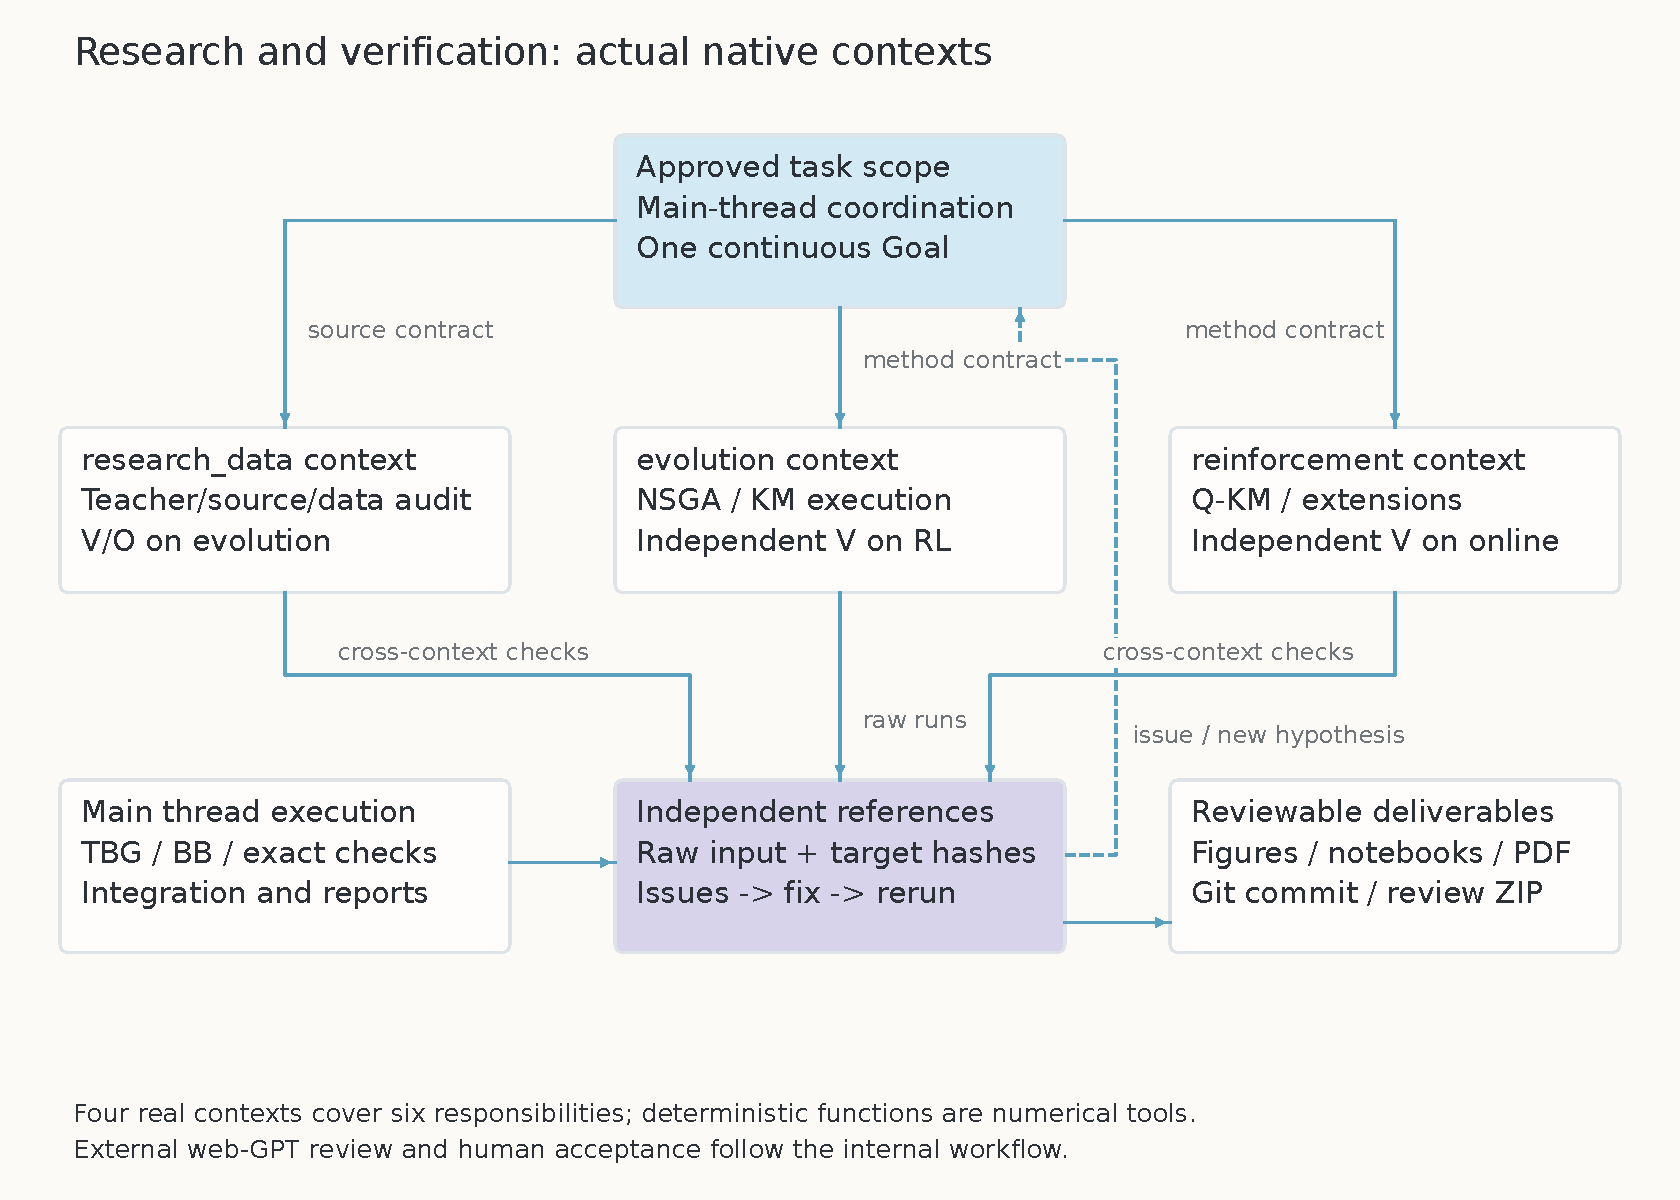
\includegraphics[width=\linewidth]{../../diagrams/research_verification_workflow.pdf}
\caption{本次真实研究与独立核验职责。四个原生上下文分时承担六类职责；箭头表示任务合同、产物和问题反馈。图解释实际技术组织，不替代原始对话UI证据。}\label{fig:processworkflow}\end{figure}

\subsection{反馈并非执行者自己的PASS}
在线分支的核验者从输入与匹配记录重新算距离、等待、唯一性和离线目标，并另写小图参考。进化核验者从原批次重解码基因，再独立求目标与HV；他发现Spacing包含了不应进入前沿的点，并提前发现初始化成本不在计时内。RL核验者没有调用作者仿真器，而是按原订单和trace重建忙闲、移动和取消，再核对Double公式和动态NSGA选点。

这些角色返回的是可定位的问题和独立读数，主线程继续落实修复，而不是收到一份审查报告就结束整个任务。没有调用付费模型API或远程GPU，也没有把最终确定性派单声称为每单一次LLM通信。原生独立上下文的真实协作与课程模型中的司机决策是两个层次。

\nextchapter\noindent {\sffamily\small\bfseries\color{C3}PART II · EXPERIMENT DECISION PROCESS}
\section{先把“比较什么”说清楚}
\subsection{材料审读先于正式计算}
Codex首先检查了已有仓库和两个新ZIP，保留原件与实验一成果。中文文件名存在混合误解码，安全提取时记录名称映射、内容哈希和无意义元数据过滤；两城市数据在多个归档里各有三份，核对后确认是重复副本，不能增加统计样本数。两份PPT共39页、两份Notebook共59 Cells分别完整审读，教师九道进阶思考题及基础讨论逐项登记。

审读暴露了两个不能靠完成代码掩盖的问题。基础Notebook有实际TODO5，但文字只说TODO1--4；BB的Assignment代码已经存在，真正的风险是把未匹配队列清空。课件还提瓶颈目标，Notebook却用总成本KM。Codex没有任选一种解释覆盖另一种，而是分别保留sum和max实现及参考。这是当前提示词已明确要求的核验，不是后来为报告补造的争论。

\subsection{低延迟曲线为何先看覆盖}
首轮55个输入、1045条方法指标中，教师场景短批次discard只服务25\%请求，司机先到的场景甚至没有服务；回收版本则能完成可用的全部供给。这个读数使图型选择有了明确目的：如果只画已服务订单的分布，丢单可能看起来更好。

Codex实际生成了完整分母ECDF和条件raincloud两种候选。前者让未服务质量保留在较低平台，后者虽能显示分布却必须另印覆盖分母。因此正式主图选择ECDF加覆盖/尾部对照，而不是因为某种图更复杂。统计单位仍是每个实例及其请求，不能把同seed内订单当作更多独立实验。

\subsection{从兜底比例到阈值诊断}
小阈值0.5/1/2有平均17\%匹配留到horizon，阈值5为7\%。Codex据此提出机制假设：过小阈值阻塞早期匹配，过大阈值又容易成为局部即时选择。随后才在3种到达顺序、相同5seed上细化阈值2/3/4/5/6/8/10/15，没有改变TBG核心或凭空增加deadline事件。

另一条负例也被保留：一个批次内最小最大成本的BBmax，在teacher seed13全天最大延迟比BBsum高2.162 min。独立核验确认实现与参考正确，因此它是未来司机选择带来的在线局限，不需要把算法改到每个指标都赢。最终独立合成seed110--114只用于确认，不重新回流选参。

\section{进化优化怎样从端点不足走到有限组合}
\subsection{先比较基础预算，再引入初始化}
进化分支先验证小图编码、解码、非支配关系与二维/三维HV，然后运行教师100种群/300代/5seed基线。18点开发批次中，NSGA-II的HV为1.090244，NSGA-III为1.077092，加权KM为1.098977。这些读数与课件参考数值分开保存，高收入端差距触发下一轮，而不是预先决定复杂混合策略更好。

先增加种群或代数，只改变一个因素。NSGA-II增种群比增代数更有利，而NSGA-III相反，说明同样约六万次评价的资源增加并非相同干预。之后才把真实KM匹配编码成初始个体，保持原100/300预算，避免把收益混在更多评价次数里。

KM单项将II/III的HV提高至1.111427/1.111494，并减小seed波动。接着测试它与种群200的一个有限组合，保留基线、增种群、KM单项和组合四个父项。组合只比KM单项增加很小HV，却增加约一倍EA评价、Spacing变差，因此没有升级最终确认预算。五个未来代理批次上只确认冻结的II原预算与KM单项，五对HV差均为正，均差0.031470。这是所测输入的支持，不是任意未来需求的理论保证。

\subsection{独立审核修正评价，不掩盖旧结果}
Research核验者发现，KM全部离散权重输出中有支配点，约$10^{-13}$求和差还会制造几乎重复的点。原始输出保持不变，报告指标统一规范去重再取非支配集，并做8/10/12位精度检查。此前Spacing不再作为当前有效评价，但旧运行没有被改写成从未发生。

初始化额外41次标量求解的成本则在正式hybrid运行前补入。这个修复影响公平预算解释，不是新增科研增益。NSGA-III在球面DTLZ2上更合适，在三目标派单细带上的优势不明显，也没有为迎合“目标更多就更好”的故事而删去。

\nextchapter\section{长期价值的收益为什么要拆开看}
\subsection{先修数据可见性，再训练}
我要求保留真实数据身份，不能把签到代理称为真实订单。数据Agent重现教师25,550条local-clock代理后，Codex主线程又取两端UTC复算，发现12对时间矛盾、6对UTC倒序。Research独立确认后，保留教师主基线，另外剔除副本做稳健性，没有偷偷统一纽约时区或重新定义原数据。

另一项更直接的修正是司机热点。原Notebook会读全量签到，本次开发只读inner签到，完整重训后也只读前70\%日期。beta扫描在验证池完成，未来测试池只在方案冻结后用于确认。300回合是实际发生的模拟训练，不是300天真实运营；这一身份贯穿曲线、表格和报告。

\subsection{Double检验没有被简化为“修复成功”}
beta1下的收入下降伴随大量非正边权。Reinforcement提出并执行Double Q手算、小例和五训练seed比较，再由独立Evolution核验。Double提高了beta1相对收入，却降低应答，拒绝的可行边比例也未降低；所以没有把理论上的过估计修正直接写成业务效果全面改善。

过程中还发现了工程混杂：更新coin与行为探索共用RNG，Double多消耗随机数会改变后续行为流。执行器暂停受影响进程，保留旧Double身份，分离随机流后重跑；Q-only数组逐项bit等价的旧结果继续按原身份引用。这个闭环由真实问题触发，不是为了让过程报告看起来更曲折。

\subsection{从无成本调度到移除边权的回退}
主动调度首先完整模拟了相邻移动、距离、时间与忙时，司机没有瞬移。无门槛版本虽然增加gross收入，却产生约5000 km/模拟日的额外空驶。看到这一负结果后，Codex才提出扣除$\lambda d$的移动门槛，并单独比较0/1/3/5，说明价值/公里的教学量纲，不假定它是真实能源价格。

原Q-KM边权与价值调度组合并未自动形成最强策略。五训练seed下，移除边权LT、保留同一个learned V做移动，gross收入反而每次都更高，因此冻结KM即时派单+门槛3的调度作为gross候选。更省空驶的门槛5保留为替代；Double和NSGA的独立作用也没有被塞进这个组合中充数。

冻结后的首批5日，候选相对Q-KM的gross差为640.81，但区间跨0；随后预登记20个新采样seed，仅确认同一冻结方法，差为435.45。额外空驶848.08 km意味着按1单位/km的情景，收入减额外调度成本之差为$-412.62$，区间也为负。这条负结果改变了解释：可以说所测gross收入增加，不能说已证明真实净收益。

\subsection{融合产生的是权衡，不是自动升级}
在独立Q-KM和NSGA成立后，才用长期边权与接驾构造前沿，并把固定膝点/约束选点带回完整仿真。约束方案降低了接驾，但收入和响应也下降；膝点更进一步牺牲服务。因此融合完成了教师加分的实测要求，却没有被称为最终全面最优。

我在执行提示词中要求保留没有收益的合法实验，这一要求在这里得到落实。具体采用、移除和停止是Codex在批准规则内依据实测作出的执行判断；没有补写成我看到每一条结果后都亲自选择，也没有把另一个角色的反馈伪装成新的人工质疑。

\nextchapter\section{把结果变成可以审核的成果}
\subsection{图文和执行证据各自核对}
正式制图实际比较了三目标3D、二维投影与平行坐标，区域V的地图小倍数与时间--区域矩阵，以及在线服务ECDF与条件分布。图型依据问题和数据选择：真实第三维才用3D；区域相邻移动需要空间关系；未匹配请求必须在统计分母中可见。不是把默认Notebook图换一种颜色就结束。

报告核验还检查图注是否对应真实样本、训练seed、验证/测试身份、波动区间和图轴。独立审稿发现，某些图只使用一个训练seed的五模拟日，不能被文字写成五训练seed；动态融合和静态前沿的预算也应分别注明。这些表述修复不重跑没有受影响的模型，但要重新构建真正的LaTeX源和PDF。

两本完成版Notebook在干净Kernel执行，保留教师Q/LT/Q-KM原断言，默认300回合没有被样本运行替代。完整参数扫描与固定结果另由可重算脚本、当前有效索引和输入/代码/产物哈希追溯。Notebook执行、重画图和报告编译是不同检查，任何一项不能冒充另外两项。

收尾时Codex把一个尚未解析命令行参数的评估入口当作支持\texttt{--help}的脚本调用，实际重放了冻结测试评估并覆盖部分文件。随后单独保存重放身份与可恢复检查点，独立Agent逐条确认95条episode/trace与原运行哈希相同，科学汇总及融合选择一致，仅运行耗时改变。未能恢复的旧逐日耗时字节如实登记；入口增加帮助参数和既存输出拒写检查。这个问题说明，命令行的无副作用行为也必须实际验证，不能靠脚本命名推断。

\subsection{公开发布边界也是一次真实反馈}
数据审计没有找到额外公开再分发许可。我把Codex的权限弹窗发给GPT询问，GPT建议采用“无额外授权，来源下载复现”，同时保留完整本地实验并限制公开数据类型。后续Codex交付记录表明，公开仓库采用了该数据边界。现有视频不能单独证明我曾逐条向Codex发出那段完整建议，因此不把GPT建议改写成我当时的逐项原话。原始签到、含数据的ZIP及可还原的逐条派生保持本地；这没有降低教师任务和实验范围。

独立包审查进一步实测：匿名的匹配选单矩阵与多条总目标可以形成满秩方程，恢复单笔fare。因此“删掉用户ID”还不够，真实EA的membership记录也从公开投影中移除，保留聚合前沿、收敛、参数、耗时、哈希和独立审核。原始完整结果没有被删除或改写。

原作者的下载渠道经过真实获取和校验。早期转换出现极少坐标末位差异，Research随后查明直接Decimal十位有效数字ROUND\_HALF\_UP和文件末尾无CRLF的规则，重新独立下载并转换后，两城市SHA与教师CSV逐字节一致。旧近似转换和失败诊断保留原身份；新输入重建仍准确标注作者来源，不倒写提供者，也不把输入一致扩大为任意环境随机产物bit一致。对数据许可的处理是发布范围控制，不是只剩总结而隐去实现。

\section{本轮保留的认识}
这次连续执行把我原先要求的“先保证正确”落实到具体对象：服务覆盖、相同目标的离线参考、共同HV、真实可行动作和物理移动成本。算法跑通以后，仍需检查比较是否成立、效果代价是什么；方法没有新增价值时，回退也构成有依据的结果。

我随后要求网页端GPT对固定提交进行二审，并在下一组真实截图中区分代码与科学成果、Process证据和最后提交的不同状态。

\end{document}
